%!TEX root = ../main.tex

\section{Choice of Moving Region Type}
\label{section:region_type_choice}

The previous section describes two different approaches to handle moving regions, each using different assumption, and each having good and bad aspects. Implementing both is not a reasonable goal for this Master thesis, and I thus had to decide which type of region I would chose to implement in MobiltyDB.

The choice was made to focus on implementing a model for manipulating moving regions of fixed-shape, based on the model presented in \cite{fmregion} and described previously. This decision was mostly arbitrary, based on personal preference, but not only. 

MobilityDB already has an underlying structure for the new data types, and this structure has to be preserved as much as possible when implementing a new feature, and this was also a factor in the final decision. The deforming region model uses a \textit{sliced representation} of the movement, whereas MobilityDB uses a \textit{sequence representation} described in \cite{mobilitydb}, so the model would have to be heavily adapted to conform to the MobilityDB structure. Using a sequence representation for storing fixed-shape moving regions seems much more straight forward.

For the rest of the thesis, we can thus assume that we are always talking about regions of fixed-shape, except if explicitly mentioned that we talk about deforming regions.

\section{Representation of Fixed-Shape Moving Regions in MobilityDB}
\label{section:internal_repr}

Now that the choice of the type of region is done, the next challenge is finding a suitable representation for these moving regions in MobilityDB. As said previously, the structure of the system has to be preserved as much as possible, which means that a temporal region type will be required for all four durations: \textit{Instant}, \textit{Instant Set}, \textit{Sequence} and \textit{Sequence Set}. These four types will be called: \textit{tgeometryinst} (for \textit{temporal geometry of instant duration}), \textit{tgeometryi}, \textit{tgeometryseq} and \textit{tgeometrys}.

\subsection{TgeometryInst}
\label{section:internal_repr_inst}

A moving region of instant duration is basically a static region, with an associated timestamp. As said in Section \ref{section:postgis}, the PostGIS type \textit{Geometry(Polygon)} will be used to describe a static region. A tgeometryinst can thus be represented similarly to any other temporal type of instant duration, that is: as a pair of value and timestamp

\[
    'v@t'
\]

, where the value is a PostGIS polygon object, and t is the timestamp. Since only one instant is present, there is no redundancy, and this is the most efficient way to store this type.

\subsection{TgeometryI}
\label{section:internal_repr_i}

As described in section \ref{section:mobilitydb_i}, a temporal value of instant set duration is simply a set of distinct timestamps stored in increasing order of their timestamp. In this case, an additional requirement on the values is present, namely the fact that all regions must be of the same shape.

A simple and naive representation for a tgeometryi is then to store all instants in the set using the previous representation. That is, store for each instant a pair of polygon and timestamp. However, since we have added the extra requirement on the polygons, namely that their shape has to be the same, we are introducing a lot of redundancy in this representation, and the storage is thus not very efficient. \\

Suppose that all the previously mentioned requirements are met, we can store the tgeometryi in a more efficient way, by storing the polygon only once, and storing the subsequent instants using only the transformation with respect to the initial instant. 

Using this representation, a tgeometryi with $n$ instants is written as:

\[
    '\{\mathcal{R}_0@t_0,\ \mathcal{T}_1@t_1,\ \mathcal{T}_2@t_2,\ ..., \ \mathcal{T}_{n-1}@t_{n-1}\}'
\]

, where $\mathcal{R}_0$ is the initial region, and $\mathcal{T}_i$ are the transformation units. \\

Section \ref{section:fixed_shape_regions} describes a possible transformation unit representing a transformation from a start to an end instant. In our case, only the end instant has to be stored, since the start instant will always be represented by the reference region $\mathcal{R}_0$ at time $t_{0}$. Since the start and end timestamp are also already stored elsewhere, namely in the timestamps $t_0$ and $t_i$, we only need to store the rotation center $C$, the translation vector $(v^x,\ v^y)$ and the rotation angle $\theta$ in the transformation unit.

\[
    \mathcal{T}_i: (C_i, v_i^x, v_i^y, \theta_i)
\]

If we want to compute the transformation unit starting from the initial and final polygons, we need to also define a rotation center for all the other parameters to be uniquely defined. For example, if we look at the start and end polygon (dark blue) shown in Figure \ref{fig:center_of_rotation}, multiple transformation units can be defined, all having the same initial and final position, but they differ in their rotation center and the path they take. The blue path has a fixed rotation center at $(3.5,\ 1)$, and there is no translation involved, while the red path uses the centroid of the polygon as rotation center, and involves a translation by 5 units along the x-axis.

\begin{figure}[h!]
    \centering
    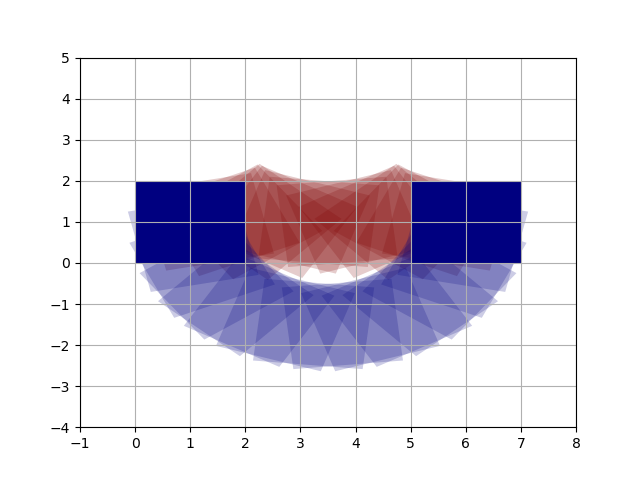
\includegraphics[width=0.75\textwidth]{images/center_of_rotation_importance.png}
    \caption{Importance of the center of rotation for a transformation.}
    \label{fig:center_of_rotation}
\end{figure}


We also know that a temporal instant set is defined only at its instants, and not in between. This means that we only care about the start and end position of a region, but we do not care about the path taken during the transformation. 

Since the decision of the rotation center only changes the path taken by the region during the transformation, the previous observation tells us that we can chose the rotation center arbitrarily when computing the transformation unit. \\

The rotation center takes a certain amount of storage space, and since we just realized that we can chose it arbitrarily, we will define the rotation center of all transformation units as being the centroid of the region at instant $t_0$. With the rotation center fixed, we can save storage space by only storing the translation vector and the rotation angle for each transformation. 

\[
    \mathcal{T}_i: (v_i^x, v_i^y, \theta_i)
\]

Using this representation, we can store a tgeometryi using minimal storage space. The two remaining challenges are: how do we compute a transformation unit starting from an initial and final polygon value, and how do we recompute the position of the region, starting from an initial polygon, and a transformation unit? The solution to these two problems is described in sections \ref{section:compute} and \ref{section:apply}. \\

As a side note, the current implementation recomputes the centroid of the polygon (center of rotation) using the PostGIS function \textit{ST\_Centroid} every time it is needed, but if we later realize that this computation is done often and is not very efficient, we can also compute it once during the input of the moving region, and then store it with the region in the first instant.

\subsection{TgeometrySeq}
\label{section:internal_repr_seq}

A temporal region of sequence duration represents the continuous movement of a region, where the position of the moving region can be retrieved at every instant between the initial and final instant. Here, we thus not only care about the position of the region at the input instants, but we also need to be able to interpolate the region between two defined instants.

As we realized previously, when computing a transformation unit starting from the initial and final position of the polygon, the choice of the rotation center defines the path taken during the movement uniquely. This means that the rotation center will have an impact on the interpolation. \\

One important assumption that was implicitly made for the tgeometryi type, is the fact that a tgeometryseq is input as a list of tgeometryinst. We are thus not getting any extra information other than the snapshots of the regions at specific instants, and, in particular, we do not know what the rotation center is for every transformation. This means that we need to define a rotation center ourselves for the transformations to be well-defined.

Having to define a rotation center ourselves has multiple consequences. First of all, since there is no way to know what the real center of rotation was simply based on the snapshots of the region at the given instants, the only solution we have is to decide on an arbitrary center of rotation. Secondly, since the arbitrary center of rotation will most probably not be the real center of rotation, there will be errors between the real path taken by the region and the interpolated path. \\

Since we know that we have to define an arbitrary center of rotation, the most obvious solution is to take the centroid of the region as the rotation center, since this point is well-defined for all regions and is easy to compute. As you might remember, this is the same solution as for tgeometryi, so we can represent a tgeometryseq in the following way:

\[
    '[\mathcal{R}_0@t_0,\ \mathcal{T}_1@t_1,\ \mathcal{T}_2@t_2,\ ..., \ \mathcal{T}_{n-1}@t_{n-1}]'
\]

, with $\mathcal{T}_i$ being the transformation with respect to $\mathcal{R}_0$:

\[
    \mathcal{T}_i: (v_i^x, v_i^y, \theta_i)
\]

The algorithmic challenges for this data type are the same as for tgeomtryi, with the addition of one problem. This problem is stated in the following way: given a polygon defined at time $t_0$, and two transformation units defined at times $t_i$ and $t_{i+1}$, both defined with respect to the initial polygon, how do we compute the position of the region at any given time $t$, where $t_i < t < t_{i+1}$? The solution to this problem is given in section \ref{section:interpolate}. \\

One last unsolved problem is the fact that the interpolated path does not exactly follow the real path taken by the moving region, when the real rotation center of the moving region is not its centroid. Solving this issue algorithmically would require us to know the real path taken by the moving region and thus the real rotation center, which, as we explained previously, is not possible when we only get snapshots of the region at distinct instants. 

The only solution to this problem without changing the assumptions made, is to give as much snapshots of the region in the input as needed to minimize the difference between interpolated path and the real path. Indeed, we can achieve any arbitrary precision by increasing the amount of instants given in the input between the initial and final position of the region. An example of how giving more instants can increase the precision of the interpolation is shown in Figure \ref{fig:num_instants_importance}. \\

\begin{figure}[h!]
\centering
\begin{subfigure}{.475\textwidth}
  \centering
  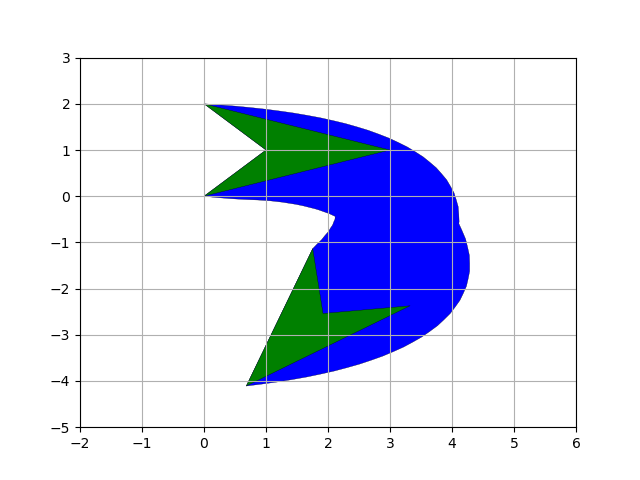
\includegraphics[width=\textwidth]{images/path_real.png}
  \caption{Real path}
  \label{fig:real_path}
\end{subfigure}
\hfill
\begin{subfigure}{.475\textwidth}
  \centering
  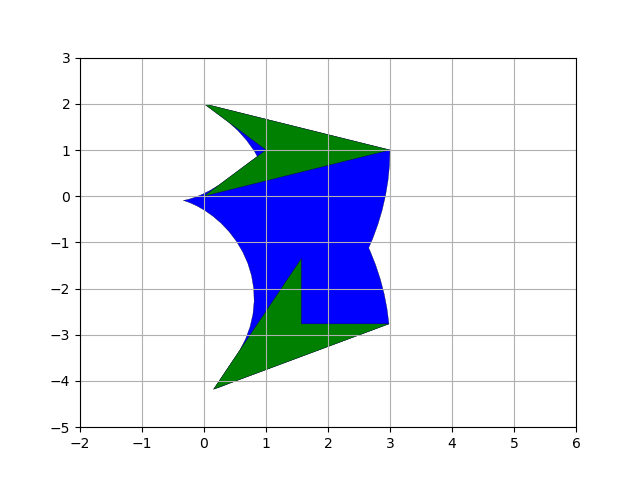
\includegraphics[width=\textwidth]{images/path_no_instants.png}
  \caption{Only start and end instant given}
  \label{fig:no_insts_path}
\end{subfigure}
\vskip\baselineskip
\begin{subfigure}{.475\textwidth}
  \centering
  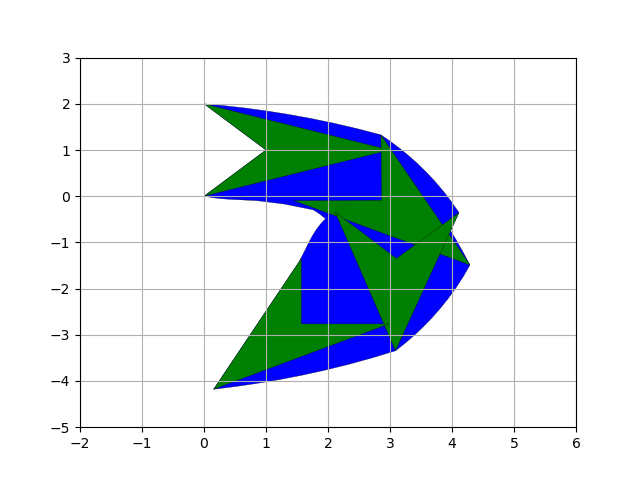
\includegraphics[width=\textwidth]{images/path_some_instants.png}
  \caption{Two intermediate instants given}
  \label{fig:some_insts_path}
\end{subfigure}
\hfill
\begin{subfigure}{.475\textwidth}
  \centering
  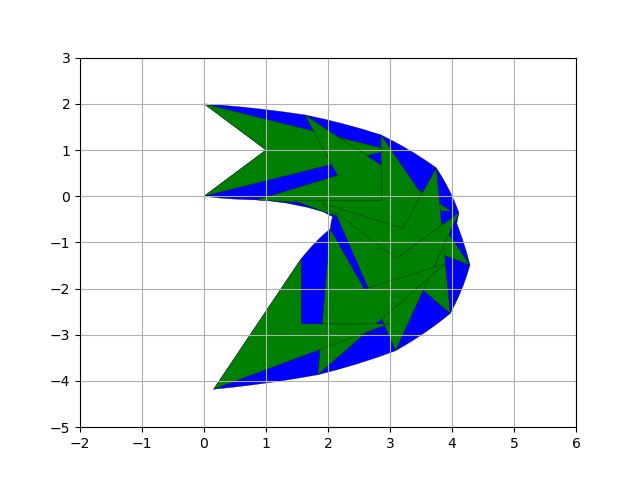
\includegraphics[width=\textwidth]{images/path_all_instants.png}
  \caption{Five intermediate instants given}
  \label{fig:all_insts_path}
\end{subfigure}
\caption[Computing the path of a moving region]{Computing the path of a moving region defined using different number of instants}
\label{fig:num_instants_importance}
\end{figure}

Figure \ref{fig:real_path} displays the real path (in blue) taken by a moving region (in green). Given only the start and end instants (in green) (Figure \ref{fig:no_insts_path}), the computed path is quite far from the reality. This computed path improves as more intermediate instants (in green) are given. The blue path shown in the figures above is computed using the traversed area function described in Section \ref{section:traversed_area}.

\subsection{TgeometryS}
\label{section:internal_repr_s}

The last type that we have to handle is tgeometrys, which is a temporal geometry of sequence set duration. The input to this type is a list of tgeometryseq. This means that we already receive some of the instants as transformations with respect to the first instant of their sequence.

For this to be a valid tgeometrys, we first need to check the fact that all regions have the same shape. Since this check was already made independently for each sequence when they were created, we thus only need to make sure that the polygons of the first instants of every sequence have the same shape. \\

Assuming that all sequences describe the movement of  polygons of the same shape, we have two possibilities to store this set of sequences. The first possibility is to store every sequence as it was received

\[
    '\{[\mathcal{R}_0^0@t_0^0,\ \mathcal{T}_1^0@t_1^0,\ ...],\ [\mathcal{R}_0^1@t_0^1,\ \mathcal{T}_1^1@t_1^1,\ ...],\ ...\}'
\]

, with every transformation $\mathcal{T}_i^j$, being defined with respect to the region $\mathcal{R}_0^j$ at the start of the sequence.

This solution is easy, since we do not have to do any more preprocessing, but it also has some redundancies, since we know that the first region of each sequence has the same shape. \\

The second possibility is thus to remove the redundancy by replacing the region values of the first instants of all sequences after the first by a transformation value. For all sequences after the first one, we have to compute the transformation of the first instant of the sequence $\mathcal{T}_0^j$ with respect to the first instant of the first sequence of the set $\mathcal{R}_0^0$. All other transformations of the sequence would have to be modified too, to have the start region being the first instant of the first sequence.

The representation would look like this:

\[
    '\{[\mathcal{R}_0^0@t_0^0,\ \mathcal{T}_1^0@t_1^0,\ ...],\ [\mathcal{T}_0^1@t_0^1,\ \mathcal{T}_1^1@t_1^1,\ ...],\ ...\}'
\]

, where every transformation $\mathcal{T}_i^j$, is defined with respect to the region $\mathcal{R}_0^0$ at the start of the first sequence.

This option requires some more preprocessing, but requires less storage space than the previous option. Another disadvantage of this method is the retrieval of a sequence in the set. This operation requires us to re-transform the whole sequence to its input representation if the required sequence is not the first one.

Depending on the use case, the average number of sequences in a set, the average number of instants in each sequence and a few more parameters, either the first option or the second option could prove to be more interesting. \\

The option that has been implemented in practice is the first one, as it seems to be the easiest one to implement, and seems to be implementable using cleaner and less code than the second option. Implementing the second option and comparing their efficiency is left as future research.

\subsection{Rtransform}

In three of the last four types, a transformation unit was used to represent an instant of a moving region more efficiently than by using a polygon. This transformation unit is stored in the database using a new type called \textit{rtransform} (short for \textit{region transformation}). As explained previously, this type only need to store information about the translation vector $(v^x,\ v^y)$ and rotation angle $\theta$ of the final value of the region, since we assume that we know what the start instant is, and we also assume the center of rotation to be the centroid of the region. Internally, all parameters of the rtransform type will be represented using the \textit{double} type.

\[
    \text{rtransform}\ \mathcal{T}: (\text{double}\ v_x,\ \text{double}\ v_y,\ \text{double}\ \theta)
\]

Since we know that rotating by $\theta$ or rotating by $\theta + 2\pi$ gives the same final result, we will add an additional constraint on the rotation angle stored in an rtransform object: $-\pi < \theta \le \pi$. This constraint allows us to compute a unique transformation unit when starting from an initial and final polygon. \\

An rtransform like this always has to be related to a polygon object, usually the polygon stored in the value of the first instant of the sequence, which will be the initial polygon. We can then apply the rtransform as explained in \ref{section:apply} to the start polygon, to retrieve the final polygon. Retrieving the polygon at an instant that is in between two stored instants, will require us to interpolate between two saved transformations to retrieve the final polygon. This interpolation method is explained in section \ref{section:interpolate}.

